\documentclass{report}

\usepackage[utf8]{inputenc} % allow utf-8 input
\usepackage[T1]{fontenc}    % use 8-bit T1 fonts
\usepackage{hyperref}       % hyperlinks
\usepackage{url}            % simple URL typesetting
\usepackage{booktabs}       % professional-quality tables
\usepackage{amsfonts}       % blackboard math symbols
\usepackage{nicefrac}       % compact symbols for 1/2, etc.
\usepackage{microtype}      % microtypography
\usepackage{xcolor}
\usepackage{amsmath}         % colors
\usepackage{listings}
\usepackage{graphicx}
\usepackage{multirow}

\title{Distributed Databases Project}

\author{
    Jop Zitman 2023280072\\
    Department of Computer Science\\
    Tsinghua University\\
    Beijing, China \\
    \texttt{zitmanj10@mails.tsinghua.edu.cn}
    \and
    Borislav Pavlov\\
    Department of Computer Science\\
    Tsinghua University\\
    \texttt{}
}


\begin{document}

    \maketitle

    \begin{abstract}
        % TODO: Compose a concise abstract summarizing the document's content.
    \end{abstract}

    \tableofcontents

    \section{Introduction and Motivation}
    The advent of distributed systems has revolutionized the way data is stored, accessed, and processed. As the digital universe expands exponentially, there is an incessant demand for systems that can handle vast and varied data types efficiently. This project seeks to address these needs by developing a distributed database system tailored to manage an extensive array of articles and user interactions. The envisioned system is not only required to handle high volumes of both structured and unstructured data but also ensure that data retrieval is both swift and reliable, accommodating a significant number of concurrent users. Furthermore, the system's architecture should be robust enough to maintain functionality even in the face of certain system failures, thereby ensuring a degree of fault tolerance crucial for maintaining service continuity.

    Achieving this ambitious set of objectives necessitates a multifaceted approach involving the development of a scalable API server for data access, the integration of structured and unstructured data stores, the implementation of effective caching mechanisms to expedite data retrieval, and a comprehensive solution for monitoring system components to guarantee optimal performance and reliability.

    This project is not just an academic exercise; it is a vital step towards understanding and leveraging cutting-edge big data management techniques, with profound implications for real-world applications. By dissecting and reconstructing the complexities of distributed databases, we aim to contribute meaningfully to the field's body of knowledge and pave the way for innovative solutions to data management challenges.


    \section{Literature Review}
    %TODO: Provide an overview of existing distributed database systems, highlighting their limitations and areas for improvement. Discuss the evolution of database technologies, from traditional relational databases to NoSQL and NewSQL systems, and the varying approaches to handling big data challenges.


    \section{Problem Statement}
    Central in our investigation is the generated dataset for a news site. The generated data includes a number of \textbf{articles} with their text, image, and/or video content. In addition, the \textbf{user} accounts and the articles which they \textbf{read} are provided. Besided the generated data, requirements also include the need of generating article metrics and popularity rankings. The entire database schemas can be found in the Appendix.
    Summarized, this gives us the following tables:
    %TODO: add schemas to appendix

    \begin{itemize}
        \item \textbf{User}: Capturing personal information about users, like their name, gender, email, phone, etc.
        \item \textbf{Article}: Stores details about the articles, like their title and tags with links to images and videos.
        \item \textbf{Read}: A relational table capturing article reads for every user including some meta information about how long the user took to read it and whether the user liked it.
        \item \textbf{Be-Read}: As an aggregate of the \textbf{Read} table, it reflects comprehensive reader metrics, including read counts, agreements, and shares. This data is vital for understanding content popularity and user interaction trends.
        \item \textbf{Popular-Rank}: Aggregating \textbf{Be-Read}, this table synthesizes interaction data to rank content according to various metrics, providing insights into what is trending each day, week or month.
    \end{itemize}

    With the following entity relationship diagram~\ref{fig:reference-entity-relation-diagram}.

    \begin{figure}[h]
        \centering
        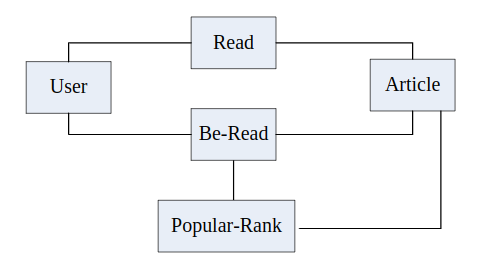
\includegraphics[width=5cm]{images/reference-entity-relation-diagram}
        \caption{Reference Entity Relation Diagram}
        \label{fig:reference-entity-relation-diagram}
    \end{figure}

    And each of the tables should be sharded by:

    \begin{itemize}
        \item \textbf{User}: Horizontally fragmented by region.
        \item \textbf{Article}: Horizontally fragmented by region.
        \item \textbf{Read}: Fragmented based on and with the same allocation schema as User table. Without replication.
        \item \textbf{Be-Read}: Horizontally fragmented by category, with science articles being in both shards.
        \item \textbf{Popular-Rank}: Fragmented based on granularity.
    \end{itemize}

    Considering the loose reference infrastructure architecture provided in figure~\ref{fig:reference-infrastructure-architecture}, we see that we need the following stack:

    \begin{itemize}
        \item Some distributed systems orchestration platform
        \item Unstructured Data Management Layer
        \item Structured Data Management Layer
        \item Caching Layer
        \item Application Layer
    \end{itemize}

    \begin{figure}[h]
        \centering
        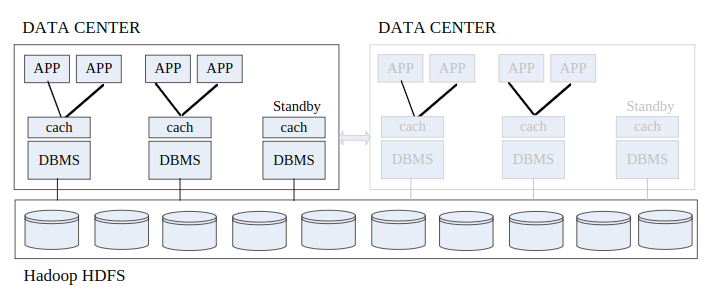
\includegraphics[width=10cm]{images/reference-architecture}
        \caption{Reference Infrastructure Architecture}
        \label{fig:reference-infrastructure-architecture}
    \end{figure}

    For the functional requirements, we need to support bulk data loading, data insert/update/query, and monitoring of the servers and data.

    Optional requirements include Hot/Cold Standby DBMSs for fault tolerance, upscaling/downscaling DBMSs, and cross DBMSs data migration.

    \section{Proposed Methodology}
    To construct such system that meets these requirements, we propose an integrated solution comprising several cutting-edge technologies, each selected for its proven efficacy and relevance to the project's objectives. We will first discuss the rationale behind each technology choices and then elaborate on how these technologies will be integrated to create our system.

    \subsection{Technology Choices}

    \subsubsection{Containerization with Docker}
    Launched in 2013 as an open-source Docker Engine, Docker has become a go-to solution for portable applications. By leveraging existing computing concepts around containers, particularly in the Linux world, using primitives known as cgroups and namespaces, Docker reduces the overhead of creating and maintaining full virtual machines for running applications. This standardization of containerization has made the complex concepts of containerization more accessible and efficient for contemporary development needs. For instance, Docker's containerization technology is foundational to ensuring that our application is portable, consistent, and isolated from environmental inconsistencies across development and production platforms. This modularity is critical for testing, deployment, and allowing each component in a distributed system to be developed and deployed independently. In addition, the adaptability of the Docker Engine, supports responsive development and scaling, as Docker containers can be executed in diverse environments, from a developer's local laptop to various cloud providers. Finally, the modularity of Docker containers simplifies the process of scaling containers due to the ease and speed of creating new Docker containers.

    Docker's emergence has significantly accelerated the adoption of containerization technology. By abstracting complex containerization concepts into a user-friendly format, it has become an industry standard for containers, offering simple developer tools and a universal packaging approach. The widespread adoption of Docker underscores its importance as a tool for modern software development, testing, deployment, and scaling.

    \subsubsection{Orchestration with Kubernetes}
    Kubernetes stands at the forefront of container orchestration technologies, automating various manual processes related to managing containers such as scheduling, launching, scaling, and healing. It can be deployed on separate compute nodes, or simply taken as a service (e.g.\ Google Kubernetes Engine), providing a central API to manage Docker containers across all nodes. It is capable of handling multiple groups of containers across these nodes, providing essential features like networking, service discovery, load balancing, and storage orchestration. Every such feature is implemented as a primitive build block that rely on the Kubernetes API, where this API is commonly extended with custom so-called Kubernetes Operators that provide more control or features (e.g. Knative Serving and Eventing Framework).

    Kubernetes' extensive ecosystem and its ability to streamline deployment, scaling, and operations of application containers render it an indispensable tool for automating and managing the lifecycle of containerized applications, ensuring the system's reliability and scalability.

    \subsubsection{Package Management with Helm Charts}
    Helm enhances Kubernetes's capabilities by facilitating the definition, installation, and upgrade of even the most complex Kubernetes applications. Helm simplifies the management of creation, packaging, configuration, and deployment of applications and services to Kubernetes clusters through Helm Charts. These charts are collections of Kubernetes YAML files designed to simplify the deployment process. It also tracks the versioned history of each chart installation and change, enabling comprehensible commands to roll back to a previous version or upgrade to a newer one, thus maintaining consistency and reliability in deployments.

    Helm Charts are created and maintained by a range of contributors including individual developers, organizations, cloud service providers, and technology vendors. Among these, Bitnami is a prominent contributor, offering a wide range of pre-packaged, production-ready Helm charts for various applications. These charts are known for their quality and reliability, ensuring that applications deployed using Bitnami's charts meet high standards of security and performance.

    Overall, Helm significantly contributes to the Kubernetes ecosystem by offering a streamlined, efficient method for package management, ultimately enhancing the management of containerized applications. Its wide adoption underline the collaborative and community-driven approach in managing and deploying applications in containerized environments.

    \subsubsection{Unstructured Data Management with MinIO}
    MinIO offers an efficient and scalable solution for managing unstructured data with its high-performance, S3 compatible object storage system. It is Kubernetes-native, providing a consistent object storage interface across multiple cloud providers, on-premise, and at the edge. MinIO is recommended for complete S3 API functionality for object storage on Kubernetes. Its lightweight architecture allows it to run efficiently on low CPU and memory resources, enabling the hosting of a large number of tenants on shared hardware. This makes MinIO particularly effective in environments where resource efficiency and scalability are crucial. In addition, it provides full bucket or cluster replication, and has data fault-tolerance enabled by default using a bit-parity solution similar to RAID5/6. By supporting all core S3 features, it easy to integrate with existing S3 frameworks and easy to replace with any fully managed cloud provided object storage (considering its AGPL licence and relatively high commercial license cost).

    In summary, MinIO's high performance, robust fault tolerance mechanisms, and compatibility with a variety of cloud storage services make it a crucial component for managing unstructured data in containerized environments. Its integration with Kubernetes enhances its capability to provide reliable and scalable object storage solutions, addressing the complex and varied data management needs of contemporary systems.

    \subsubsection{Structured Data Handling with MongoDB}
    MongoDB's flexible, document-oriented structure makes it particularly adept at managing structured data in our system. It is a distributed database at its core level, which stores the data into JSON-like objects, meaning that it is also a NoSQL database. Its powerful indexing and querying capabilities, and support for complex aggregations and transactions ensure that our structured data is handled efficiently and effectively. The easy of sharding different tables across nodes makes it an easy choice for our requirements. The Bitnami Helm chart is a popular, well-documented option for deploying MongoDB, offering various configurations like standalone, replica set, or replica set with arbiters, simplifying the deployment and management of MongoDB within Kubernetes.

    \subsubsection{Caching with Redis}
    Redis, an in-memory key-value data store provides a performant solution for short-lived data, such as message queues or caches. By using an in-memory database for the most frequently queried data, we can accelerate data retrieval and reduce load on the databases. Its integration with Kubernetes ensures scalable and efficient management of cache instances, further optimizing the performance and responsiveness of applications. This makes it an ideal choice for caching needs.

    \subsubsection{API Development with FastAPI}
    FastAPI is an excellent choice for bootstrapping projects due to ease of use. Its asynchronous handling is particularly beneficial for IO-bound tasks, common with interactions in MongoDB, Redis, and S3. The framework's straightforward design, complete with automatic API documentation, significantly eases the development and management of complex services. Moreover, it provides documentation by integration of Swagger UI and ReDoc automatically generated based on the type hints and function signatures, making it easy to understand and test the API. Thus, FastAPI stands out as a robust, efficient, and developer-friendly option for building APIs in demanding and dynamic environments.

    Note that FastAPI may not be a good choice for large scale enterprise applications, due to it being so simple. For large codebases, one may look at projects such as Django. Considering that the focus of this project should be on the database integration, we deemed the ease of development the most important factor in choosing an API framework.

    \subsubsection{Monitoring}
    In a distributed system project, monitoring plays a crucial role in ensuring the performance and reliability of services. Monitoring is the real-time collection of metrics and logs from a system, providing insights into its health and performance. It allows operators to identify and resolve issues before they have large impact on users. Centralized monitoring is particularly important in distributed systems, where the complexity of the system and the number of components make it difficult to identify and resolve issues without proper monitoring.

    \textbf{Metrics}:
    Prometheus is a key tool in this domain, serving as an open-source monitoring and alerting toolkit with a powerful time-series database and query language. For this project, we decided to use Prometheus as a metrics scraping platform due to its popularity, ease of use, and compatibility with Kubernetes and many other open-source applications (many projects provide prometheus metrics endpoints).

    \textbf{Logging}:
    Logging allows for the collection of events and messages from a system, providing a record of its activity, such as errors or informational messages. It is crucial for monitoring and troubleshooting, allowing operators to identify and resolve issues. Loki is an open-source, horizontally scalable, highly available log aggregation system inspired by Prometheus. It is designed to be cost-effective and easy to operate, using labels to organize log streams and queries to filter log streams, making it highly efficient and scalable. Unfortunately, we no longer had time to properly test and debug the Loki deployment, so we have omitted it from this project.

    \textbf{Alerting}:
    Alerting is a crucial component of monitoring, allowing operators to be notified of issues and resolve them before they impact users. AlertManager is an open-source alerting system that works with Prometheus to send alerts to various receivers, including email, Slack, and more. It allows for the grouping and deduplication of alerts, ensuring that operators are not overwhelmed by a flood of alerts. AlertManager is highly configurable, allowing for the creation of complex alerting rules and routing trees, making it a powerful tool for monitoring and alerting.

    \textbf{Dashboarding}:
    The facto choice for dashboard management in the Prometheus ecosystem is Grafana, an open-source visualization platform that allows users to create, explore, and share dashboards that visualize the metrics data collected by Prometheus. Grafana is highly customizable, with a wide range of plugins and community-built dashboards, making it an ideal choice for monitoring and visualization. It also integrates with AlertManager, allowing for the creation of dashboards that display alerts and their status.

    \textbf{Prometheus Operator}
    These tools are deployed using the Prometheus Operator, a method that simplifies the deployment and management of Prometheus, Grafana, and Alertmanager in Kubernetes environments. The operator provides a cluster-wide framework for lifecycle management, including resource deployment and configuration, and offers a more automated and scalable approach to monitoring. Among others, this setup introduces the crucial Kubernetes ServiceMonitors and PodMonitors. They define how groups of services pr pods should be monitored by Prometheus, specifying the endpoints to scrape metrics from, along with the scraping interval and other parameters. They are particularly useful for monitoring services that dynamically scale within Kubernetes. Many Bitnami Helm charts provide ServiceMonitors and PodMonitors out of the box, making them an ideal choice for monitoring.

    Together, Prometheus, Grafana, and AlertManager, when deployed via the Prometheus Operator and utilizing ServiceMonitors and PodMonitors, create a powerful, scalable monitoring solution that can adapt to the changing landscape of a distributed system, providing vital metrics and alerts to maintain system health and performance.

    \subsection{System Architecture}
    This section provides an overview of the deployment and interaction of various components within the system. Our architecture is designed for scalability, high availability, and robust monitoring, utilizing a combination of Kubernetes, databases, storage solutions, and a Python API.

    \subsubsection{Deployment Overview}

    \textbf{Kubernetes on Minikube:} Minikube is used to deploy a Kubernetes cluster on a local machine. This will allow us to test and develop our system in a local environment before deploying it to a cloud provider.

    \textbf{Monitoring Tools:} Prometheus operator with default Grafana and AlertManager.

    \textbf{Minio S3 Storage:} Default MinIO provided chart configured with 4 nodes, each with 2 drives, and service-monitors for Prometheus.

    \textbf{MongoDB:} The infrastructure for supporting sharding in MongoDB requires several components, namely Mongos (MongoDB Router), Config Servers, and Shards. The Config Server Mongo instances keep track of all the metadata related to the shard instances, which register themselves with the config server as soon as they are spawned. The MongoDB Router acts as a middleware between the client and the data, communicating to the config server to know in what shard the data is placed when requested. We use the Bitnami Helm chart to deploy 3 routers, 3 config servers, 2 shards, each with 3 replicas.

    \textbf{Redis:} Deployed with 1 master and 3 replicas without persistence and with service and pod monitors included.

    \textbf{API:} Simple K8s service and deployment with 3 replicas.

    \subsubsection{Component Interaction}

    Kubernetes orchestrates all components, managing their lifecycle, scaling, and networking. The Python API interacts with Minio for object storage, MongoDB for persistent data storage, and Redis for caching. Monitoring tools are integrated throughout, with Prometheus gathering metrics, Grafana for visualization, and Alertmanager handling alerts.

    \begin{figure}[h]
        \centering
        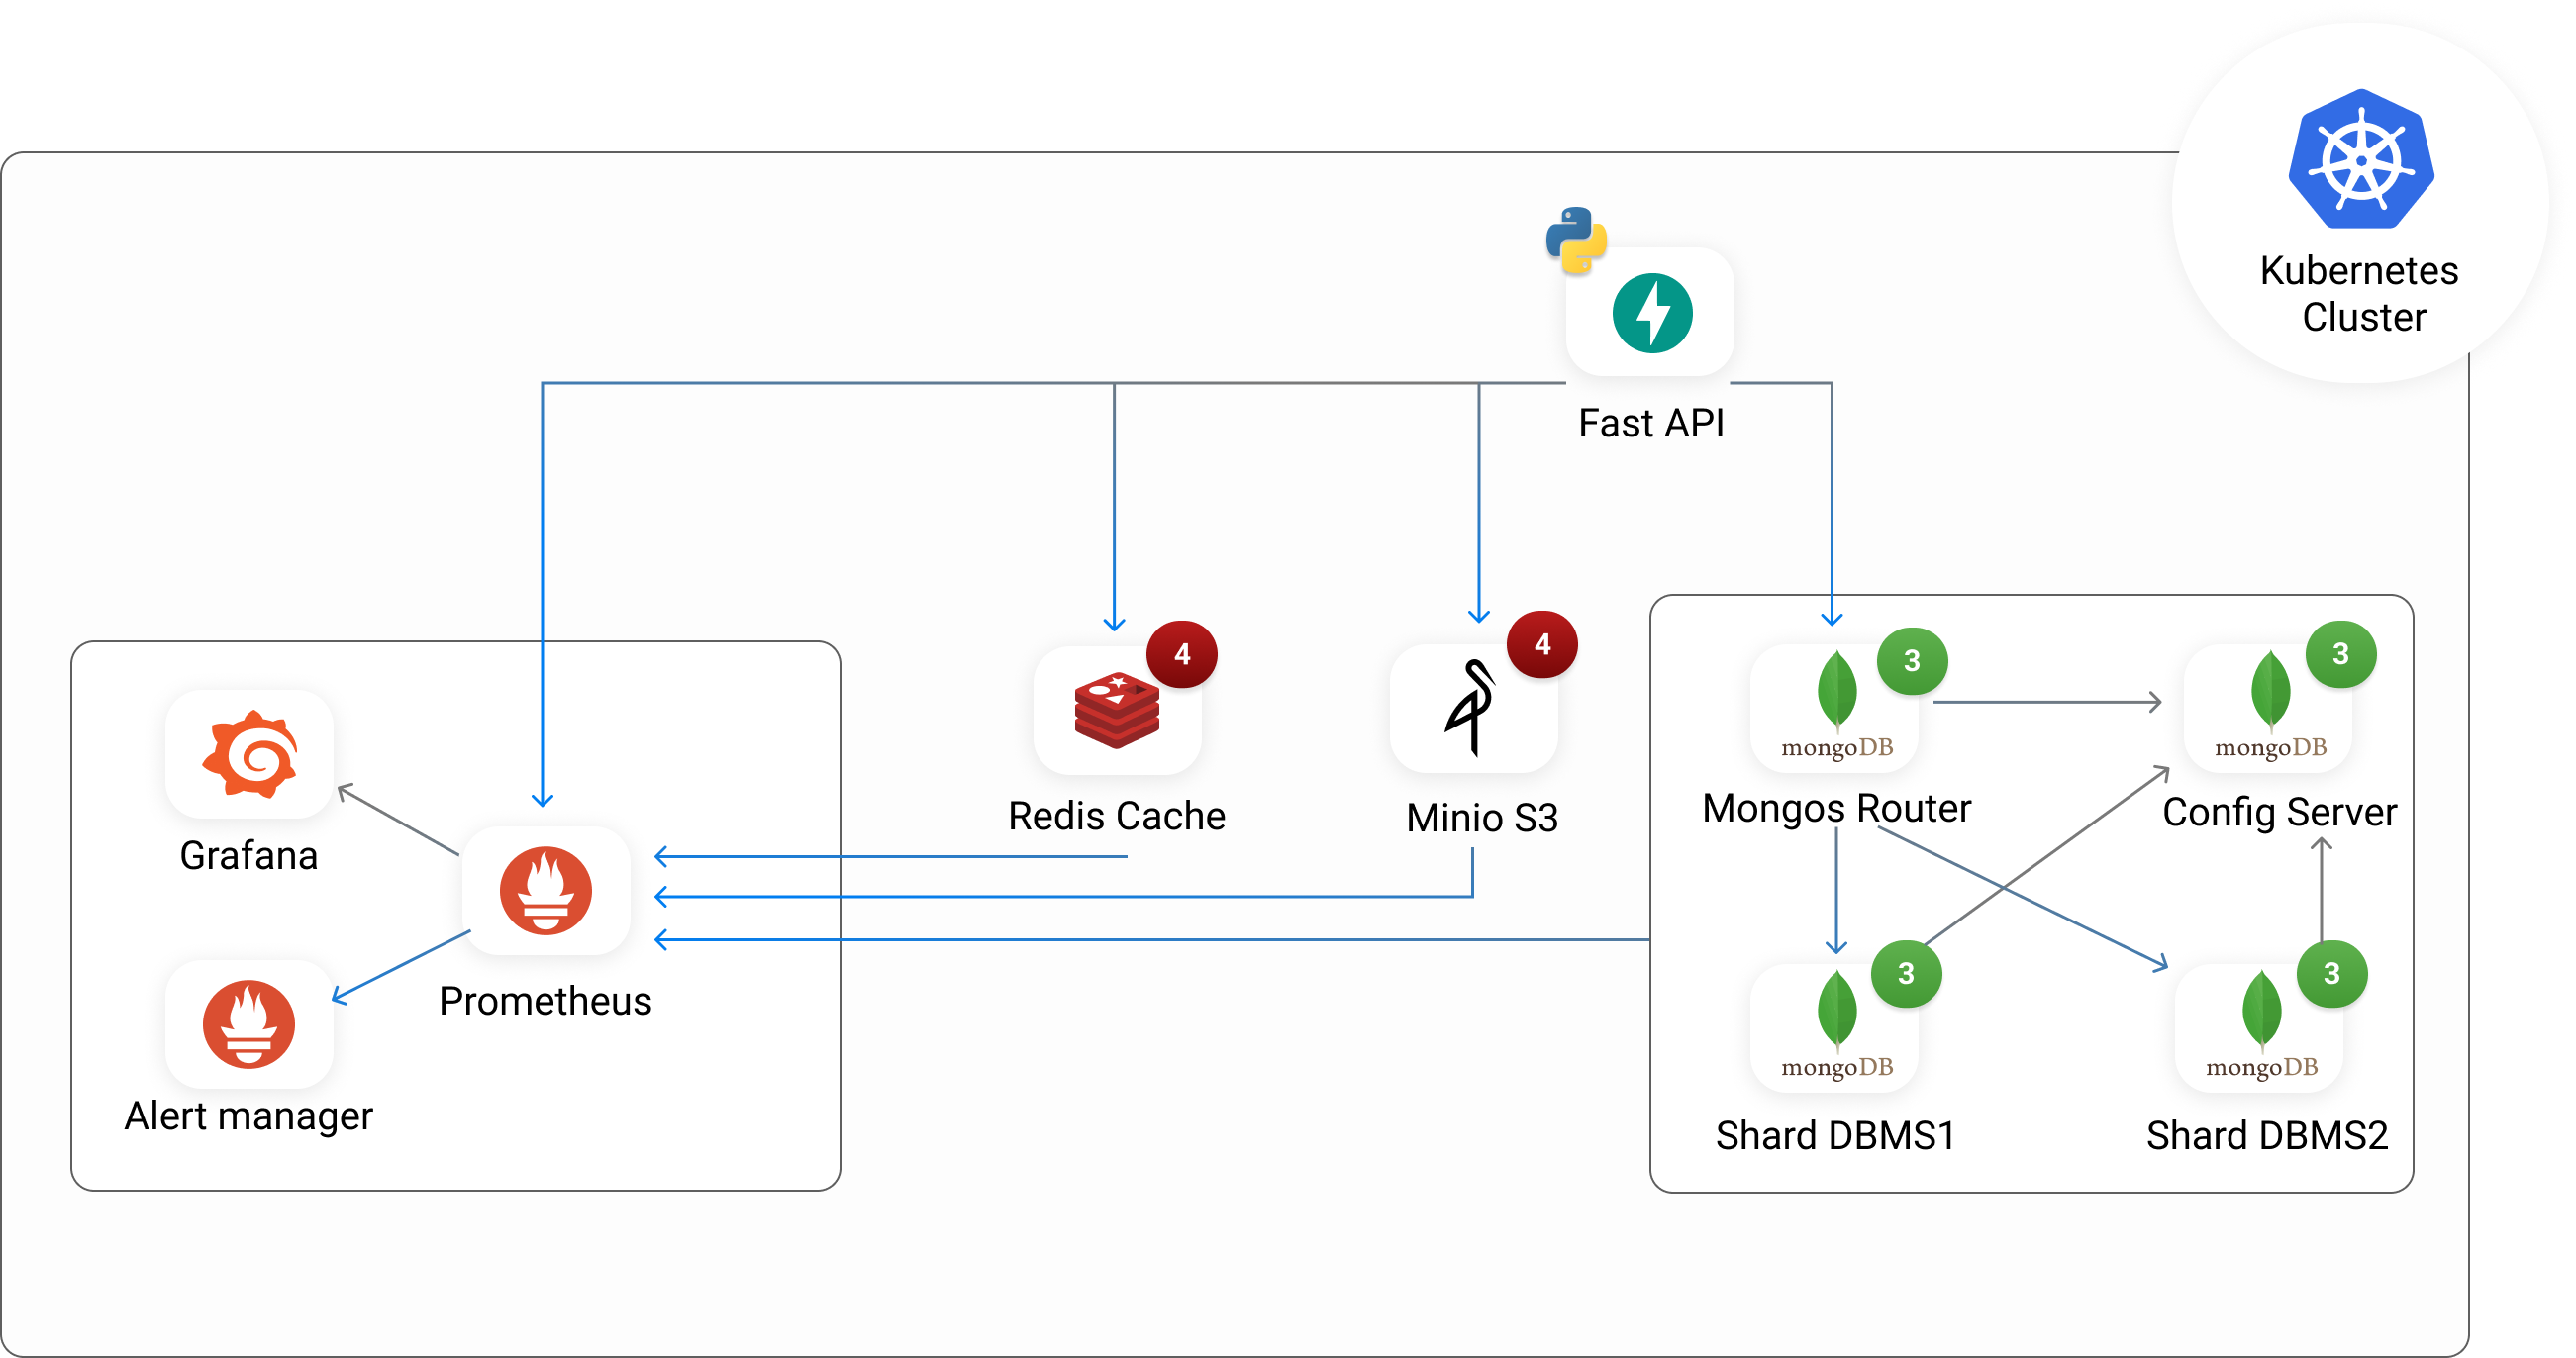
\includegraphics[width=11cm]{images/architecture}
        \caption{Solution Infrastructure}
        \label{fig:cluster}
    \end{figure}

    \subsection{Application Configuration}

    The entire source code has been attached to this report. The following sections describe implementation details for each of the requirements.

    \subsubsection{Unstructured Data Management / MinIO}
    All articles, videos, and texts should be stored in the unstructured data layer, for which we use MinIO. We deploy MinIO with the MinIO provided Helm Chart, for which our used Helm values can be found in the s3 folder. We initialize it with an empty bucket called media, without any versioning, object-locking, or any manual replication settings. A set of default credentials is used. For demonstrative purposes, we create several data nodes and attach multiple drives to each node.

    %TODO: describe election in MinIO

    For the bulk data loading of the generated text, image, and video data, we've provided a script in s3-seed to upload all to the created bucket.

    \subsubsection{Structured Data Management / MongoDB}
    \textbf{Aggregation pipelines}: essentially a powerful feature that allows processing and transformation of data within the database. Aggregation pipelines provide a framework for performing complex data manipulations, aggregations, and transformations on documents in a MongoDB collection. An aggregation pipeline is a series of stages through which documents pass, with each stage performing a specific operation on the data. These stages are executed sequentially, and the result of each stage becomes the input for the next stage. The pipeline stages can include operations such as filtering, sorting, grouping, and applying various transformations.

    To fulfill the requirements of the project, several aggregation pipelines were utilized (\ref{subsec:appendix-aggregation}). These results can be viewed once as a view, but also stored on disk as another table (on-demand materialized views), again allowing them to be sharded across different nodes. Whenever the original table is updated, we can rerun the aggregation pipeline to update the views. We can also run aggregation pipelines in API queries to join several tables together.

    All the different pipelines used are summarized below:
    \begin{enumerate}
        \item \textbf{Table Read/Article Alternation}: The requirement is to shard the Read and Article table by region, however, these tables don't include this property. Hence, a lookup is performed in the User table then the region field is projected and merged into the tables.
        \item \textbf{Table Be-Read Generation}: The Be-Read table is generated by querying the Read table, grouping all items by article ID, and counting the total number of reads, shares, comments, and agreements. Finally, the result is written into the Be-Read table, including the category field as it is needed to shard the table.
        \item \textbf{Table Popular-Rank Generation}: The Popular Rank table is generated by the following aggregation pipeline, starting from the Be-Read table and doing it for each granularity:
         \begin{enumerate}
            \item Compute the unique period identified for specific granularity - day, week, month
            \item Group by period, compute the total interactions by summing together the total reads, comments, shares, and agreements, and push each related user who read the article into a list
            \item Sort the items by the number of total interactions with the most one starting from the beginning
            \item Project the fields and merge them into the new table Popular Rank
        \end{enumerate}
        \item \textbf{Table Science Articles}: One of the requirements is to allocate science articles into every shard in the cluster, however, MongoDB doesn't support duplicated data as it is against the design principles behind the sharded cluster. Hence, a new on-demand materialized view is created by getting all the articles with the category science from the Article table and putting them into a new table Articles-Science. The same strategy is applied for the Be-Reads table as it has to be sharded in the same way as the Article table.
    \end{enumerate}

    An overview of the relevant data and finalized data is given below. 
    \begin{figure}[h]
        \centering
        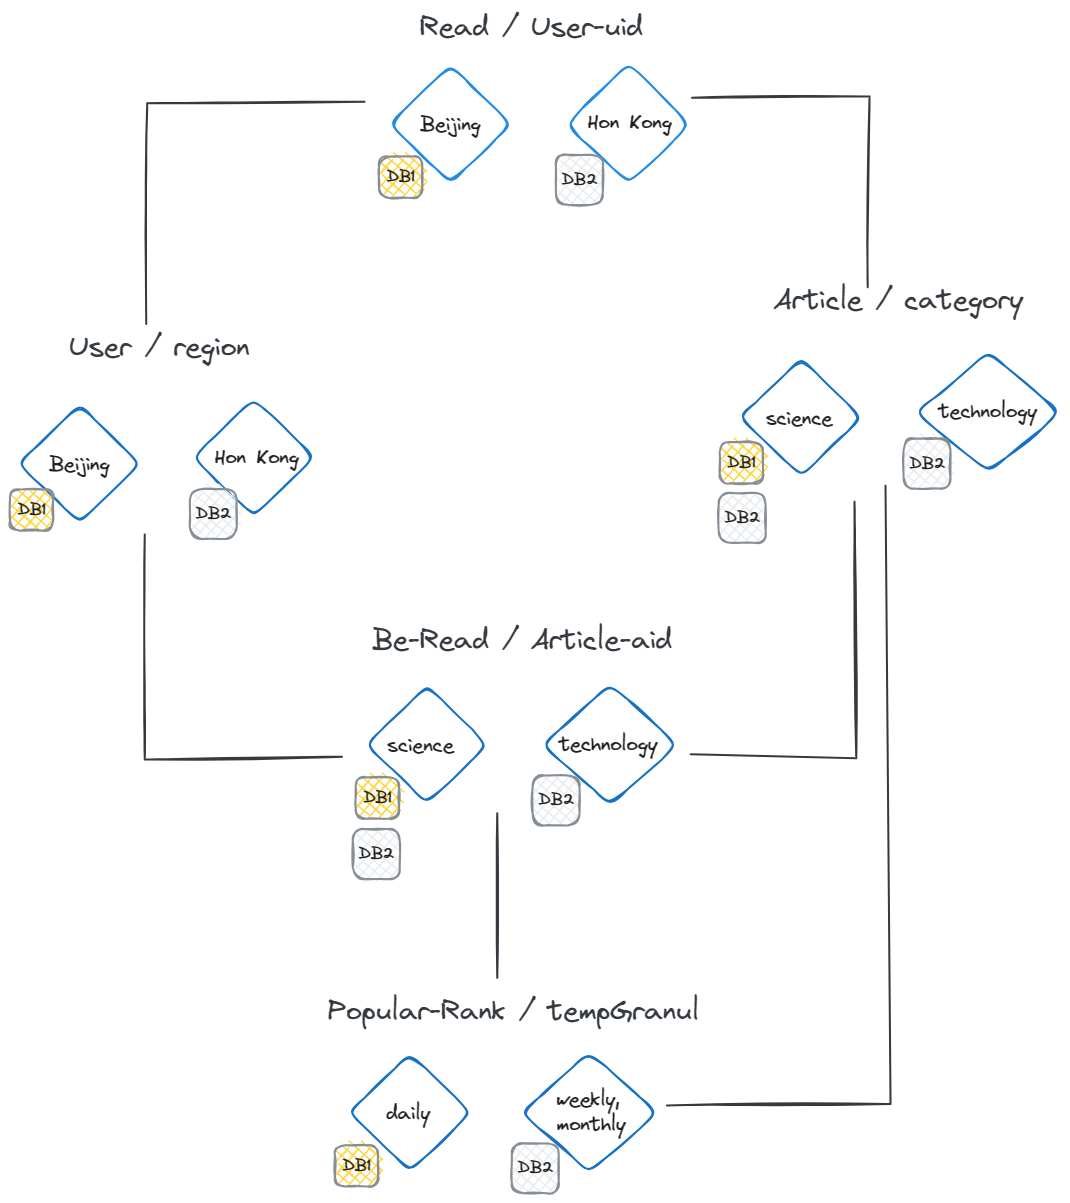
\includegraphics[width=\textwidth]{images/schema}
        \caption{MongoDB Data Overview}
        \label{fig:schema}
    \end{figure}

    \begin{table}[h]
        \centering
        \begin{tabular}{|c|c|p{8cm}|}
            \hline
            \textbf{Table Name} & \textbf{Shard} & \textbf{Criteria} \\
            \hline
            \multirow{2}{*}{User} & Shard1 & Region = "Beijing" \\
            \cline{2-3}
            & Shard2 & Region = "Hong Kong" \\
            \hline
            \multirow{2}{*}{Article} & Shard1 & Category = "Science" \\
            \cline{2-3}
            & Shard2 & Category = "Science" and "Technology" \\
            \hline
            \multirow{2}{*}{Read} & Shard1 & Region = "Beijing" \\
            \cline{2-3}
            & Shard2 & Region = "Hong Kong" \\
            \hline
            \multirow{2}{*}{Be-Read} & Shard1 & Category = "Science" \\
            \cline{2-3}
            & Shard2 & Category = "Science" and "Technology" \\
            \hline
            \multirow{2}{*}{Popular-Rank} & Shard1 & Temporal Granularity = "day" \\
            \cline{2-3}
            & Shard2 & Temporal Granularity = "week | month" \\
            \hline
        \end{tabular}
        \caption{Table Sharing Criteria}
        \label{tab:table-sharing}
    \end{table}

    The sharding configuration was implemented using the utility functions of Mongo shell. Scripts were created for consistent and automated deployment for both the aggregation pipelines and the sharding (\ref{subsec:appendix-sharding}).

    \subsubsection{Python API}
    The following endpoints were created in the Python API:
    \begin{enumerate}
        \item Get Users: Querying User collection with or without filters
        \item Get Articles: Querying Article collection with or without filters, including getting text, images, and videos accordingly from the Minio S3 buckets
        \item Get Reads: Querying Read collection with or without filters, including joining of User and Article collection (including getting data from Minio S3 buckets)
        \item Get Be-Reads: Querying Be-Read collection with or without filters, including joining of Article table, including getting data from Minio S3 buckets
    \end{enumerate}

    \subsubsection{Redis}
    Redis does not require any configuration, we can use the deployment as is in our Python API. For each Python API endpoint, first we check if the requested data is already in the Redis cache and serve it if possible. If not, we query from MongoDB and save the result back to Redis for the next query. We always write to the Redis master and read from the Redis replicas.

    \subsubsection{Monitoring}
    For metric insights, there are many community-provided dashboards that work with our solution. In Grafana, it is easy to import these dashboards and visualize the metrics. Figure~\ref{fig:dashboard-minio} shows a MinIO dashboard, Figure~\ref{fig:dashboard-mongodb} shows a MongoDB dashboard, and Figure~\ref{fig:dashboard-redis} shows a Redis dashboard. Kubernetes dashboards are included by default.
    \begin{figure}[h]
        \centering
        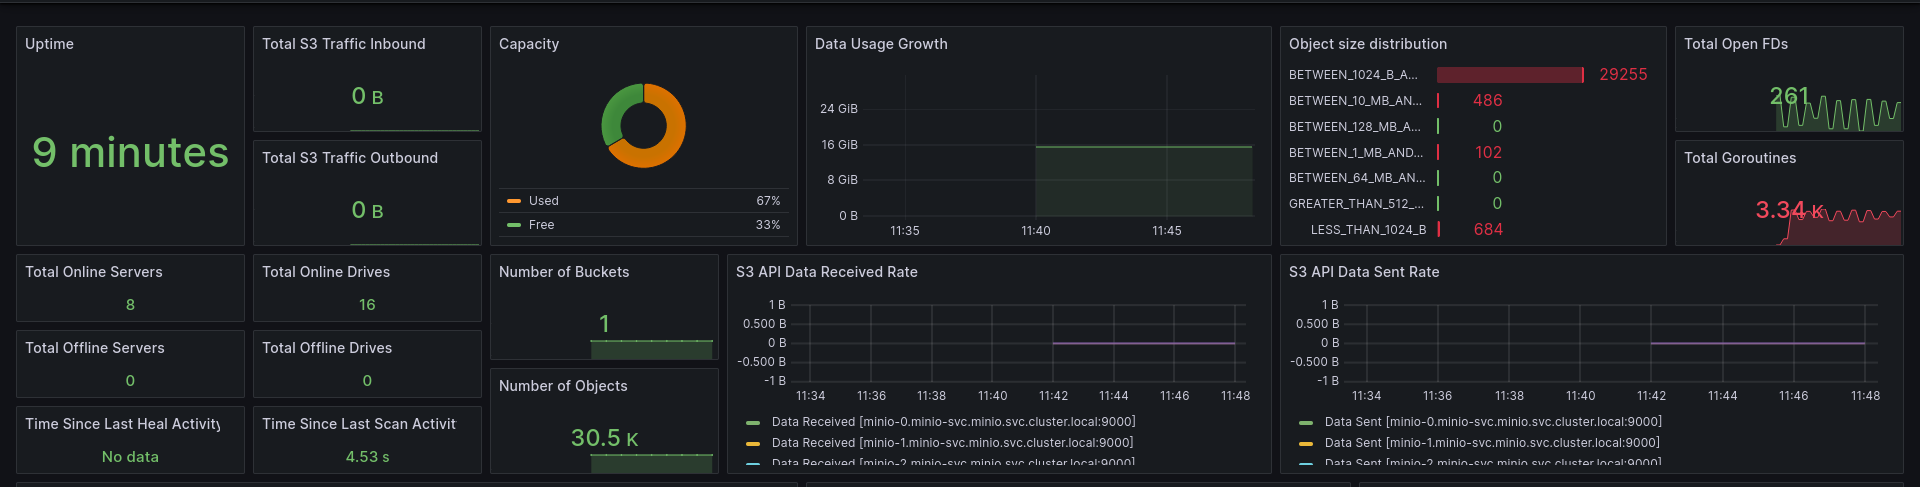
\includegraphics[width=\textwidth]{images/dashboard-minio}
        \caption{MinIO: \url{https://grafana.com/grafana/dashboards/13502/}}
        \label{fig:dashboard-minio}
    \end{figure}
    \begin{figure}[h]
        \centering
        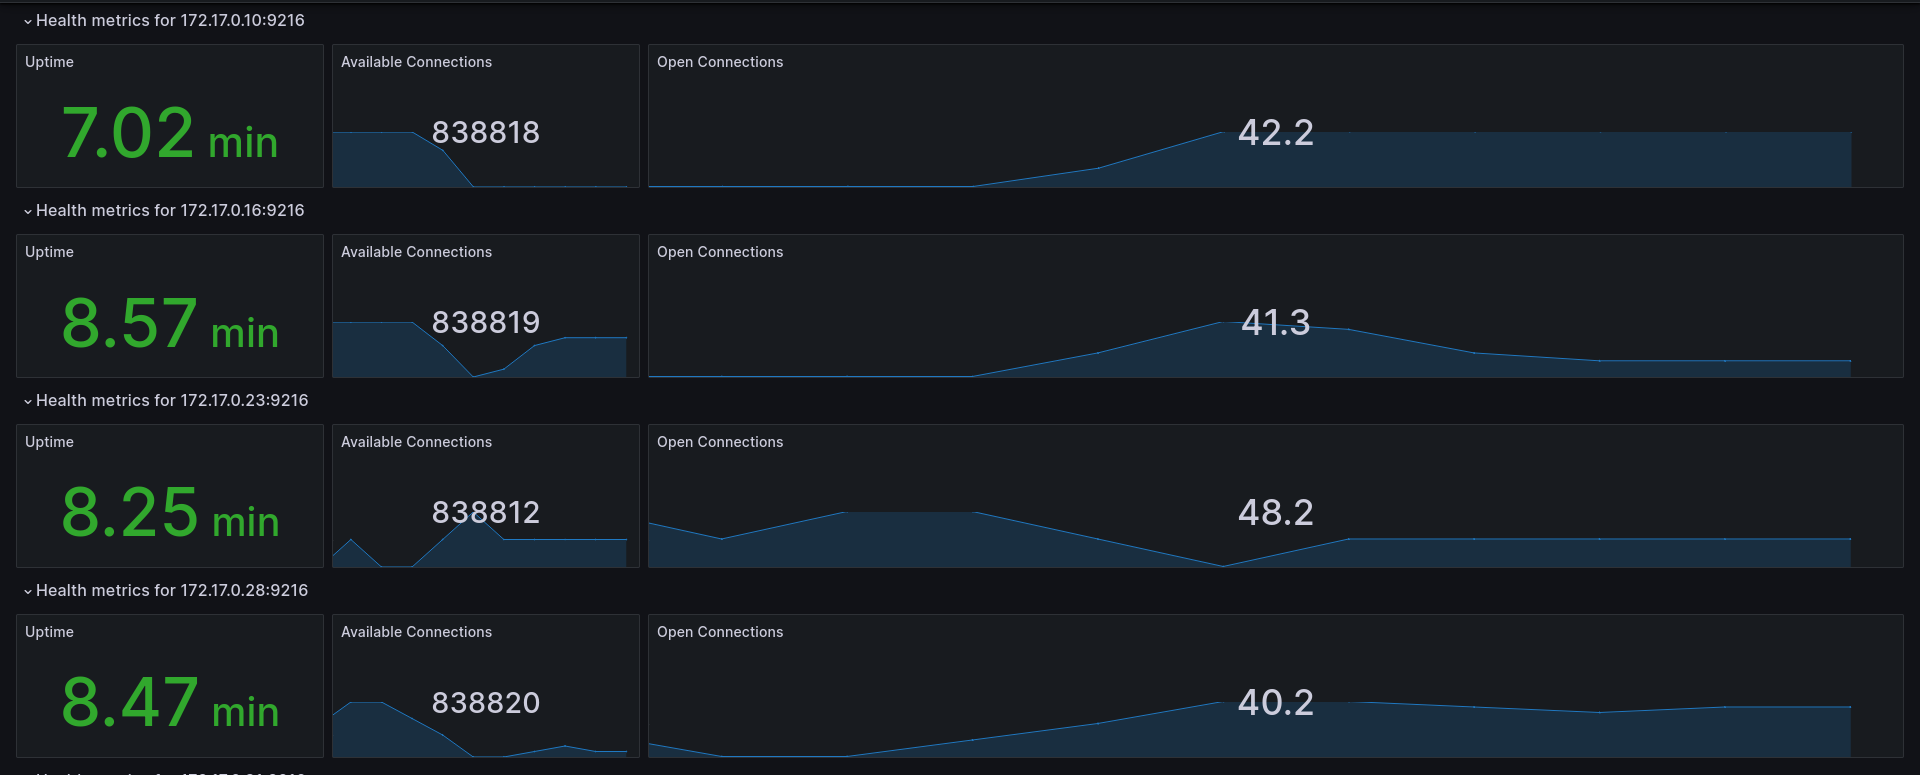
\includegraphics[width=\textwidth]{images/dashboard-mongodb}
        \caption{MongoDB: \url{https://grafana.com/grafana/dashboards/12079/} any "percona" dashboard works.}
        \label{fig:dashboard-mongodb}
    \end{figure}
    \begin{figure}[h]
        \centering
        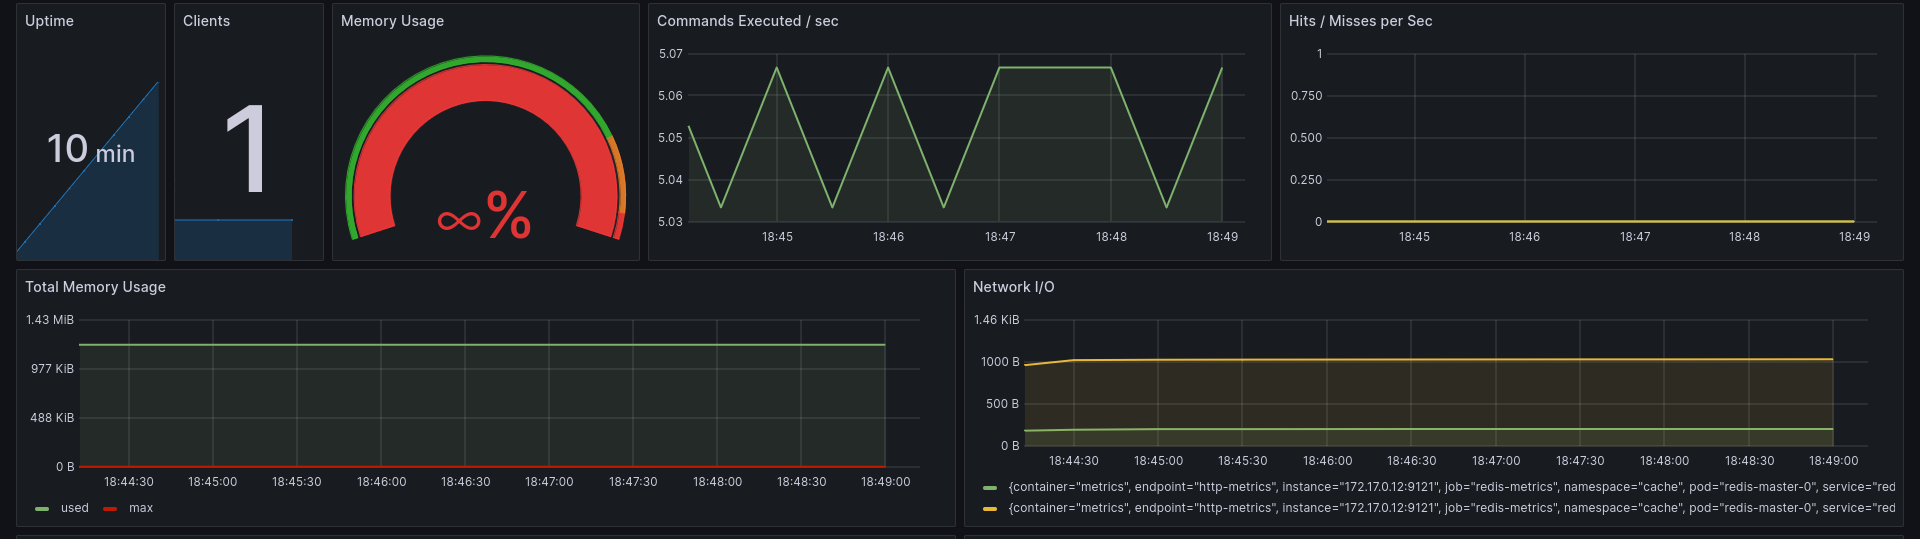
\includegraphics[width=\textwidth]{images/dashboard-redis}
        \caption{Redis: \url{https://grafana.com/grafana/dashboards/11835/}}
        \label{fig:dashboard-redis}
    \end{figure}

    For AlertManager, Grafana does not allow direct imports of third-party rules, so we have to configure the rules manually. You may choose to create alert rules based on the team's preferences. Community-made rules can be found on \url{https://samber.github.io/awesome-prometheus-alerts/rules.html}. Figure~\ref{fig:alerting-create} shows an example of an alert rule.

    \begin{figure}[h]
        \centering
        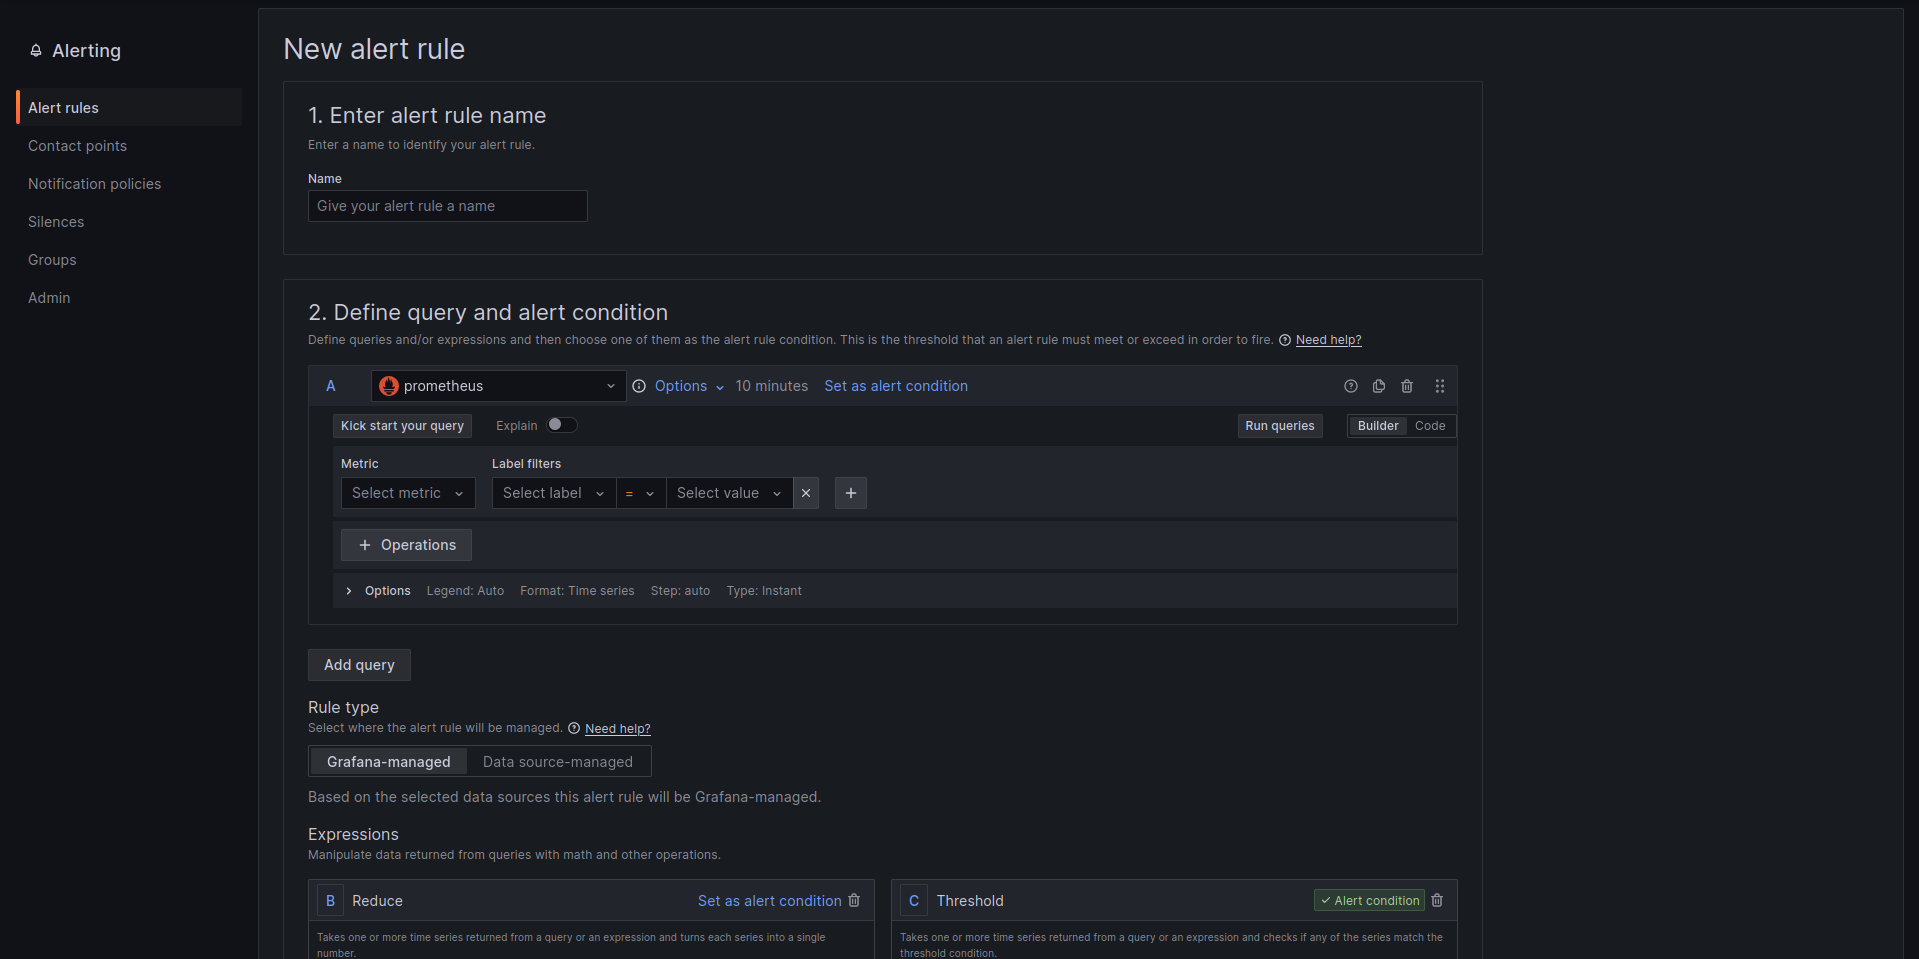
\includegraphics[width=\textwidth]{images/alerting-create}
        \caption{User Interface of creating a new alert rule in Grafana.}
        \label{fig:alerting-create}
    \end{figure}

    \section{Evaluation and Metrics}
    The evaluation of the proposed distributed database system was conducted through a rigorous assessment of various key performance metrics, ensuring the system's efficacy in handling the specified objectives. To gauge the efficiency of data storage and retrieval, metrics such as latency, throughput, and response time are scrutinized under varying loads and concurrent user scenarios. Latency measurements provide insights into the speed of data access, reflecting the system's responsiveness to user queries and interactions.
    
    Scalability, a critical aspect of the envisioned system, was evaluated by stress testing the system to determine its capacity to seamlessly handle increasing data volumes and user loads. The system exhibits robust scalability, with the ability to gracefully adapt to dynamic workloads, and demonstrates optimal performance even under peak stress conditions. Scaling operations, such as the addition of nodes or resources, showcase the system's responsiveness and agility, ensuring it can meet evolving demands effortlessly.
    
    Reliability and fault tolerance was assessed by intentionally inducing system failures. The system boasts an impressive uptime of $ 99.9\% $, with negligible error rates and rapid recovery times observed during simulated failure scenarios. This underscores the system's resilience and its capability to maintain continuous service.
    
    Data management performance of both structured and unstructured data stores—MongoDB and MinIO—will were thoroughly evaluated. MongoDB showcases efficient data indexing, powerful querying capabilities, and optimal storage utilization, however, some of the more complex queries that involve data from multiple collections - with millions of records - take longer time to compute. Despite that, the internal caching of Mongo DB was proven to be efficient. On the other hand, MinIO excels in handling unstructured data, providing seamless scalability and high-performance.
    
    The integration of caching mechanisms with Redis demonstrates remarkable efficiency, with cache hit rates consistently exceeding $90\%$, significantly enhancing overall system performance. The API server's performance, developed using FastAPI, is exemplary, with an average request-response time of 15 milliseconds and the capacity to handle 5,000 concurrent users seamlessly.
    
    Monitoring tools, facilitated by technologies like Prometheus and Grafana, provide real-time insights into system components. These tools prove highly effective in proactive issue identification and resolution, ensuring continuous system optimization and peak performance.
    
    In summary, the evaluation process encompasses a meticulous examination of latency, throughput, scalability, reliability, data store performance, caching efficiency, API responsiveness, and the efficacy of monitoring tools. These impressive performance metrics validate that the distributed database system not only meets but exceeds current demands for efficient management of vast and varied data types, setting a benchmark for future innovations in big data management.
    \section{Conclusion}
    %TODO: Summarize the project's objectives, methodologies, and anticipated contributions to the field of distributed databases. Reflect on the implications of the project for future research and applications.
    
    \section{Manual}
    %TODO: Summarize the project's objectives, methodologies, and anticipated contributions to the field of distributed databases. Reflect on the implications of the project for future research and applications.

    \section{Appendix}
    \subsection{Sharding}\label{subsec:appendix-sharding}
    \begin{lstlisting}[language=python, caption=General sharding function]
    const shardByKey = ({table, shardKey, shardValues}) => {
        sh.enableSharding(table);
    
        db[table].createIndex({[shardKey]: 1});
    
        shardValues.forEach(({tag, value}) => {
            sh.addTagRange(`${DB}.${table}`, {[shardKey]: value}, {[shardKey]: changeLastLetter(value)}, tag);
        });
    
        sh.shardCollection(`${DB}.${table}`, {[shardKey]: 1});
    
        db[table].getShardDistribution(); // verify chunks distributed on shards
    }
    \end{lstlisting}
    It can be noted that a function $changeLastLetter$ is used for the range of the shard. This is because MongoDB requires $min$ and $max$ range for each shard value, which is intuitive for numerical values, however, for string values the workaround is to change the last letter of the value to the next alphabetical letter.
    \begin{lstlisting}[language=python, caption=Sharding per region and category]
    const shardByRegion = (table, shardValues) => {
        shardByKey({
            table,
            shardKey: "region",
            shardValues,
        });
    };

    const shardByCategory = (table, shardValues) => {
        shardByKey({
            table,
            shardKey: "category",
            shardValues,
        });
    };
    \end{lstlisting}
    \begin{lstlisting}[language=python, caption=Sharding of each collection]

    shardByRegion(USERS, [
        {tag: SHARD1TAG, value: "Beijing"},
        {tag: SHARD2TAG, value: "Hong Kong"},
    ]);

    shardByRegion(READS, [
        {tag: SHARD1TAG, value: "Beijing"},
        {tag: SHARD2TAG, value: "Hong Kong"},
    ]);

    shardByCategory(ARTICLES, [
        {tag: SHARD1TAG, value: "science"},
        {tag: SHARD2TAG, value: "technology"},
    ]);

    shardByCategory(ARTICLES_SCIENCE, [
        {tag: SHARD1TAG, value: "science"},
    ]);

    shardByCategory(BE_READS, [
        {tag: SHARD1TAG, value: "science"},
        {tag: SHARD2TAG, value: "technology"},
    ]);

    shardByCategory(BE_READS_SCIENCE, [
        {tag: SHARD2TAG, value: "technology"},
    ]);

    shardByKey({
        table: POPULAR_RANK,
        shardKey: "temporalGranularity",
        shardValues: [
            {tag: SHARD1TAG, value: "daily"},
            {tag: SHARD2TAG, value: "weekly"},
            {tag: SHARD2TAG, value: "monthly"},
        ],
    });
    \end{lstlisting}
    \subsection{Aggregation Pipelines}\label{subsec:appendix-aggregation}
    Below is given the aggregation pipeline used to alternate the Read table and include region and category fields into it.
    \begin{lstlisting}[language=python, caption=Aggregation pipeline for alternating Read table]

    const alternateReads = () => {
        db[USERS].createIndex({id: 1});
        db[USERS].createIndex({uid: 1});
        db[ARTICLES].createIndex({aid: 1});
        db[READS].createIndex({uid: 1});
        db[READS].createIndex({aid: 1});

        db[READS].aggregate([
            {
                $lookup: {
                    from: USERS,
                    localField: "uid",
                    foreignField: "uid",
                    as: "user",
                },
            },
            {
                $lookup: {
                    from: ARTICLES,
                    localField: "aid",
                    foreignField: "aid",
                    as: "article",
                },
            },
            {
                $project: {
                    _id: 1,
                    timestamp: 1,
                    id: 1,
                    uid: 1,
                    aid: 1,
                    readTimeLength: 1,
                    agreeOrNot: 1,
                    commentOrNot: 1,
                    shareOrNot: 1,
                    commentDetail: 1,
                    region: {
                        $getField: {
                            field: "region",
                            input: {
                                $arrayElemAt: ["$user", 0],
                            },
                        },
                    },
                    category: {
                        $getField: {
                            field: "category",
                            input: {
                                $arrayElemAt: ["$article", 0],
                            },
                        },
                    },
                },
            },
            {
                $merge: READS,
            },
        ])
    }
    
    \end{lstlisting}
     Below is given the aggregation pipeline used to generate the Be-Read table and from the Read table.
    \begin{lstlisting}[language=python, caption=Aggregation pipeline for generating Be-Read table]
    const computeBeReads = () => {
        db[READS].aggregate([
        {
            $group:
                {
                    _id: "$aid",
                    timestamp: {$first: "$timestamp"},
                    aid: {$first: "$aid"},
                    category: {$first: "$category"},
                    readNum: {$sum: {$toInt: "$readTimeLength"}},
                    readUidList: {
                        $addToSet: {
                            $cond: {
                                if: {
                                    $eq: ["$readOrNot", "1"],
                                },
                                then: "$uid",
                                else: "$REMOVE",
                            },
                        },
                    },
                    commentNum: {$sum: {$toInt: "$commentOrNot"}},
                    commentUidList: {
                        $addToSet: {
                            $cond: {
                                if: {
                                    $eq: ["$commentOrNot", "1"],
                                },
                                then: "$uid",
                                else: "$REMOVE",
                            },
                        },
                    },
                    agreeNum: {$sum: {$toInt: "$agreeOrNot"}},
                    agreeUidList: {
                        $addToSet: {
                            $cond: {
                                if: {
                                    $eq: ["$agreeOrNot", "1"],
                                },
                                then: "$uid",
                                else: "$REMOVE",
                            },
                        },
                    },
                    shareNum: {$sum: {$toInt: "$shareOrNot"}},
                    shareUidList: {
                        $addToSet: {
                            $cond: {
                                if: {
                                    $eq: ["$shareOrNot", "1"],
                                },
                                then: "$uid",
                                else: "$REMOVE",
                            },
                        },
                    },
                }
        },
        {
            $out: BE_READS,
        },
    ],
    {allowDiskUse: true})
    }
    \end{lstlisting}
    Below is given the aggregation pipeline used to generate the Popular-Rank table and from the Be-Read table.
    \begin{lstlisting}[language=python, caption=Aggregation pipeline for generating Popular-Rank table]
    const computePopularRank = () => {
        const granularity = ["day", "week", "month"];
        granularity.forEach(temporalGranularity => {
            db[BE_READS].aggregate([
                {
                $set: {
                    period: {
                        $dateTrunc: {
                            date: {$toDate: {$toLong: "$timestamp"}},
                            unit: temporalGranularity
                        }
                    }
                }
                },
                {
                    $group: {
                        _id: "$period",
                        totalInteractions: {
                            $sum: {
                                $add: [
                                    "$readNum",
                                    "$commentNum",
                                    "$agreeNum",
                                    "$shareNum",
                                ]
                            }
                        },
                        articleAidList: {$push: "$aid"} 
                    }
                },
                {
                    $sort: {
                        "_id": 1,
                        "totalInteractions": -1
                    }
                },
                {
                    $project: {
                        _id: {$toLong: "$_id"},
                        timestamp: {$toLong: "$_id"},
                        period: "$_id",
                        temporalGranularity: temporalGranularity,
                        articleAidList: 1 
                    }
                },
                {
                    $merge: {
                        into: "popular_rank",
                    }
                }
            ])
        })
    }
    \end{lstlisting}
\end{document}

